%standard 3.1

%start_of_questions

%new_question
%%%%%%%%%%%%%%%%%%%%%
	% Problem 1
	% Difficulty: 1
%%%%%%%%%%%%%%%%%%%%%
	\item  
		Use the following code to answer the below questions\\
		\mbox{ \hspace*{0.25in}	\lstinputlisting[language=Python]{./code/c1.py}}
		\begin{enumerate}
			\item Find four values of my\_var so each of the four assignment statements will be executed: 
				each value should cause one assignment statement to be executed.
			\item Find four ranges of my\_var values that will cause each of the four assignment 
				statements to be executed.
		\end{enumerate}


%new_question
%%%%%%%%%%%%%%%%%%%%%
	% Problem 2
	% Difficulty: 1
%%%%%%%%%%%%%%%%%%%%%
	\item  
		In your own words, describe the difference in logic of the following two sets of code:\\
		\begin{minipage}{.5\textwidth}
			(a) \mbox{\hspace*{2em} \lstinputlisting[language=Python]{./code/c2a.py}}
		\end{minipage}
		\begin{minipage}{.5\textwidth}
			(b) \mbox{\hspace*{2em} \lstinputlisting[language=Python]{./code/c2b.py}}
		\end{minipage}


%new_question
%%%%%%%%%%%%%%%%%%%%%
	% Problem 3
	% Difficulty: 1
%%%%%%%%%%%%%%%%%%%%%
	\item  
		When driving in a car and approaching a traffic control light, \textit{green} means go, 
		\textit{yellow} means yield, and \textit{red} means stop.  Assuming there is a variable 
		named \textit{light\_color}, write a program that prints either the word \textit{go}, 
		\textit{yield}, or \textit{stop} depending of the value of \textit{light\_color}.  
		Let the user input the value of \textit{light\_color}.



%new_question
%%%%%%%%%%%%%%%%%%%%%
	% Problem 8
	% Difficulty: 1
%%%%%%%%%%%%%%%%%%%%%
	\item  
		Write a program that asks the user for three numbers, and then determines (and outputs) 
		which of the numbers is the largest.  Do not use the built-in function \textit{max}().\\
		For example, \\ \ \hfill
		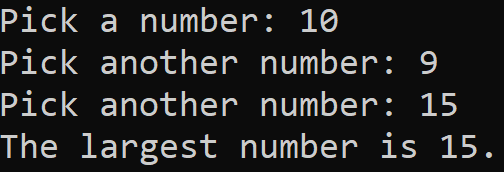
\includegraphics[height = 0.6in]{./imgs/largest_ex1.PNG} \hfill
		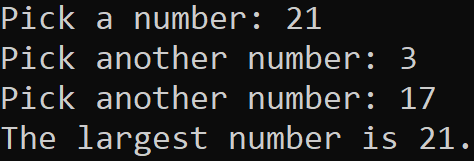
\includegraphics[height = 0.6in]{./imgs/largest_ex2.PNG} \hfill \ 



%new_question
%%%%%%%%%%%%%%%%%%%%%
	% Problem 9
	% Difficulty: 1
%%%%%%%%%%%%%%%%%%%%%
	\item  
		Write a program that asks the user for three numbers, and then determines (and outputs)
		which of the numbers is the smallest.  Do not use the built-in function \textit{min}().\\
		For example, \\ \ \hfill
		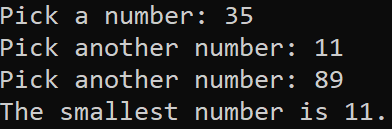
\includegraphics[height = 0.6in]{./imgs/smallest_ex1.PNG} \hfill
		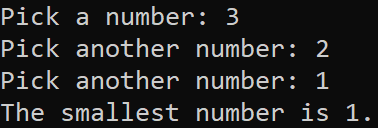
\includegraphics[height = 0.6in]{./imgs/smallest_ex2.PNG} \hfill \ 




%new_question
%%%%%%%%%%%%%%%%%%%%%
	% Problem 11
	% Difficulty: 1
%%%%%%%%%%%%%%%%%%%%%
	\item  
		(Game: heads or tails)  Write a program that lets the user guess whether the flip of a coin 
		results in heads or tails.  The program randomly generates an integer 0 or 1, which 
		represents head or tail.  The program prompts the user to enter a guess and reports whether 
		the guess is correct or incorrect.\\
		Hint: These should be your first two lines of code.
		\begin{verbatim}
		    from random import randint
		    value = randint(0,1) #picks a random integer. Either 0 or 1.
		\end{verbatim}




%new_question
%%%%%%%%%%%%%%%%%%%%%
	% Problem 14
	% Difficulty: 1
%%%%%%%%%%%%%%%%%%%%%
	\item  
		Write a program that prompts the user for a letter and checks whether the letter is a vowel 
		or consonant.  A vowel should output \textit{\csq{vowel}}, and a consonant should output 
		\textit{consonant}.  You may assume only lower case letters. Below is sample output.\\
		Hint: In the English language, a, e, i, o, and u are the vowels.
	
		\begin{figure}[h]
		\centering
			\begin{minipage}{.5\textwidth}
			\centering
				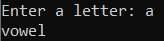
\includegraphics[scale=1.2]{./imgs/vowelYesAlt.png}
			\end{minipage}%
				%
			\begin{minipage}{.5\textwidth}
			\centering
				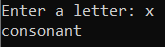
\includegraphics[scale=1.1]{./imgs/vowelNoAlt.png}
			\end{minipage}
		\end{figure}





%new_question
%%%%%%%%%%%%%%%%%%%%%
	% Problem 16
	% Difficulty: 1
%%%%%%%%%%%%%%%%%%%%%
	\item  
		At the local ice cream store they have 3 flavors, which are Vanilla, Chocolate, and 
		Strawberry. Write a program that ask the user which type of ice cream they want and print 
		the flavor they selected. However, if they picked a flavor that is not available, inform 
		the user of such.
	
		\hfill 
		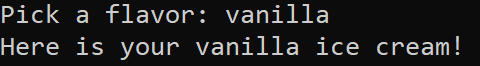
\includegraphics[width = 2.5in]{./imgs/iceCreamFlavors1.PNG} \hfill 
		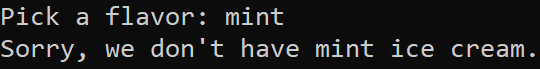
\includegraphics[width = 2.5in]{./imgs/iceCreamFlavors2.PNG} \hfill \ 




%new_question
%%%%%%%%%%%%%%%%%%%%%
	% Problem 19
	% Difficulty: 1
%%%%%%%%%%%%%%%%%%%%%
	\item  
		%https://edabit.com/challenge/8pDH2SRutPoaQghgc
		Luke Skywalker has friends and family, but he is getting older and having trouble 
		remembering them all.  Write a program that Luke (the user) can input a name and it 
		outputs the relation defined in the table below.
		\begin{center}
		\begin{tabular}{|l|l|} \hline
			Person 		& Relation \\ \hline \hline
			Darth Vader	& Father \\ \hline
			Leia		& Sister \\ \hline
			Han			& Brother in law\\ \hline
			R2D2		& Droid \\ \hline
		\end{tabular}\\ \hspace*{1in} *If he types any other name, report \csq{unknown}.
		\end{center}
		


%end_of_questions




